\documentclass[letterpaper,12pt]{article}
\usepackage[utf8]{inputenc}
\usepackage[spanish]{babel}
\usepackage[a4paper,margin=2.5cm]{geometry}
\usepackage{hyperref}
\usepackage{pdfpages}
\usepackage{setspace}

\hypersetup{
    colorlinks=true,
    linkcolor=black,
    urlcolor=blue,
    pdftitle={Reporte Final Integrado - Proyecto Olist},
    pdfauthor={Marcelo de la Quintana, Gaston Nina, Gerick Toro}
}

\begin{document}

\begin{titlepage}
    \centering
    {\Large Universidad Mayor de San Andres\par}
    \vspace{0.5cm}
    {\large Maestria en Inteligencia Artificial y Ciencia de Datos\par}
    \vspace{1.5cm}
    {\Huge \textbf{Reporte Final Integrado}\par}
    \vspace{0.4cm}
    {\Large Proyecto de Identificacion de Clientes Premium sobre Olist\par}
    \vspace{1.5cm}
    {\large Modulo de Implementacion de Soluciones de Inteligencia Artificial\par}
    \vspace{1.5cm}
    {\large
        Marcelo de la Quintana\par
        Gaston Nina\par
        Gerick Toro\par
    }
    \vfill
    {\large Junio 2026\par}
\end{titlepage}

\tableofcontents
\newpage

\section*{Presentacion}
\addcontentsline{toc}{section}{Presentacion}
Este documento consolida en un unico entregable los cuatro informes tecnicos del proyecto. Para preservar fidelidad academica y trazabilidad, cada sprint se incorpora como su reporte oficial completo, manteniendo su estructura, tablas, figuras y conclusiones originales.

\section{Sprint 1: Perfilado, EDA y Baseline}

\includepdf[pages=-,pagecommand={}]{../../sprint_01/informes/sprint_01_reporte.pdf}

\section{Sprint 2: Pipeline y Features}
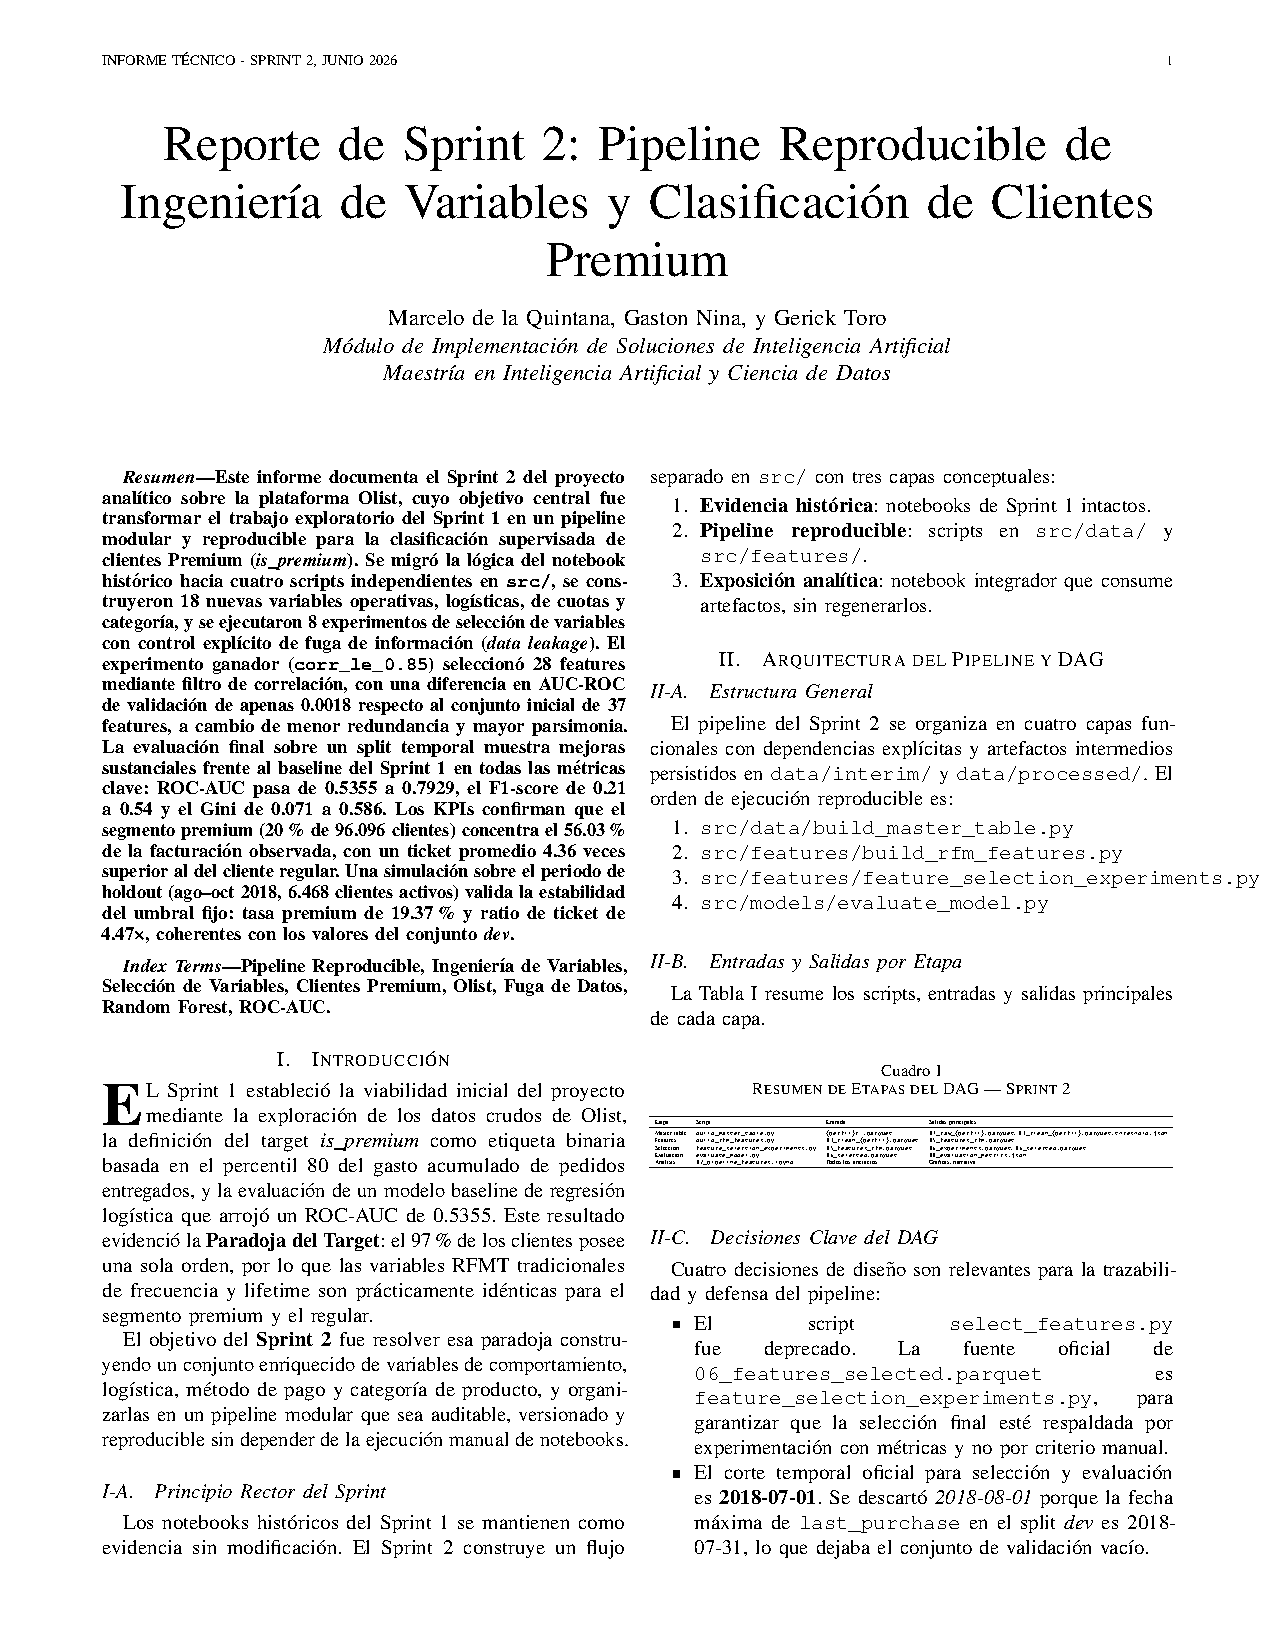
\includepdf[pages=-,pagecommand={}]{../../sprint_02/informes/sprint_02_reporte.pdf}

\section{Sprint 3: Modelo Final y HPO}
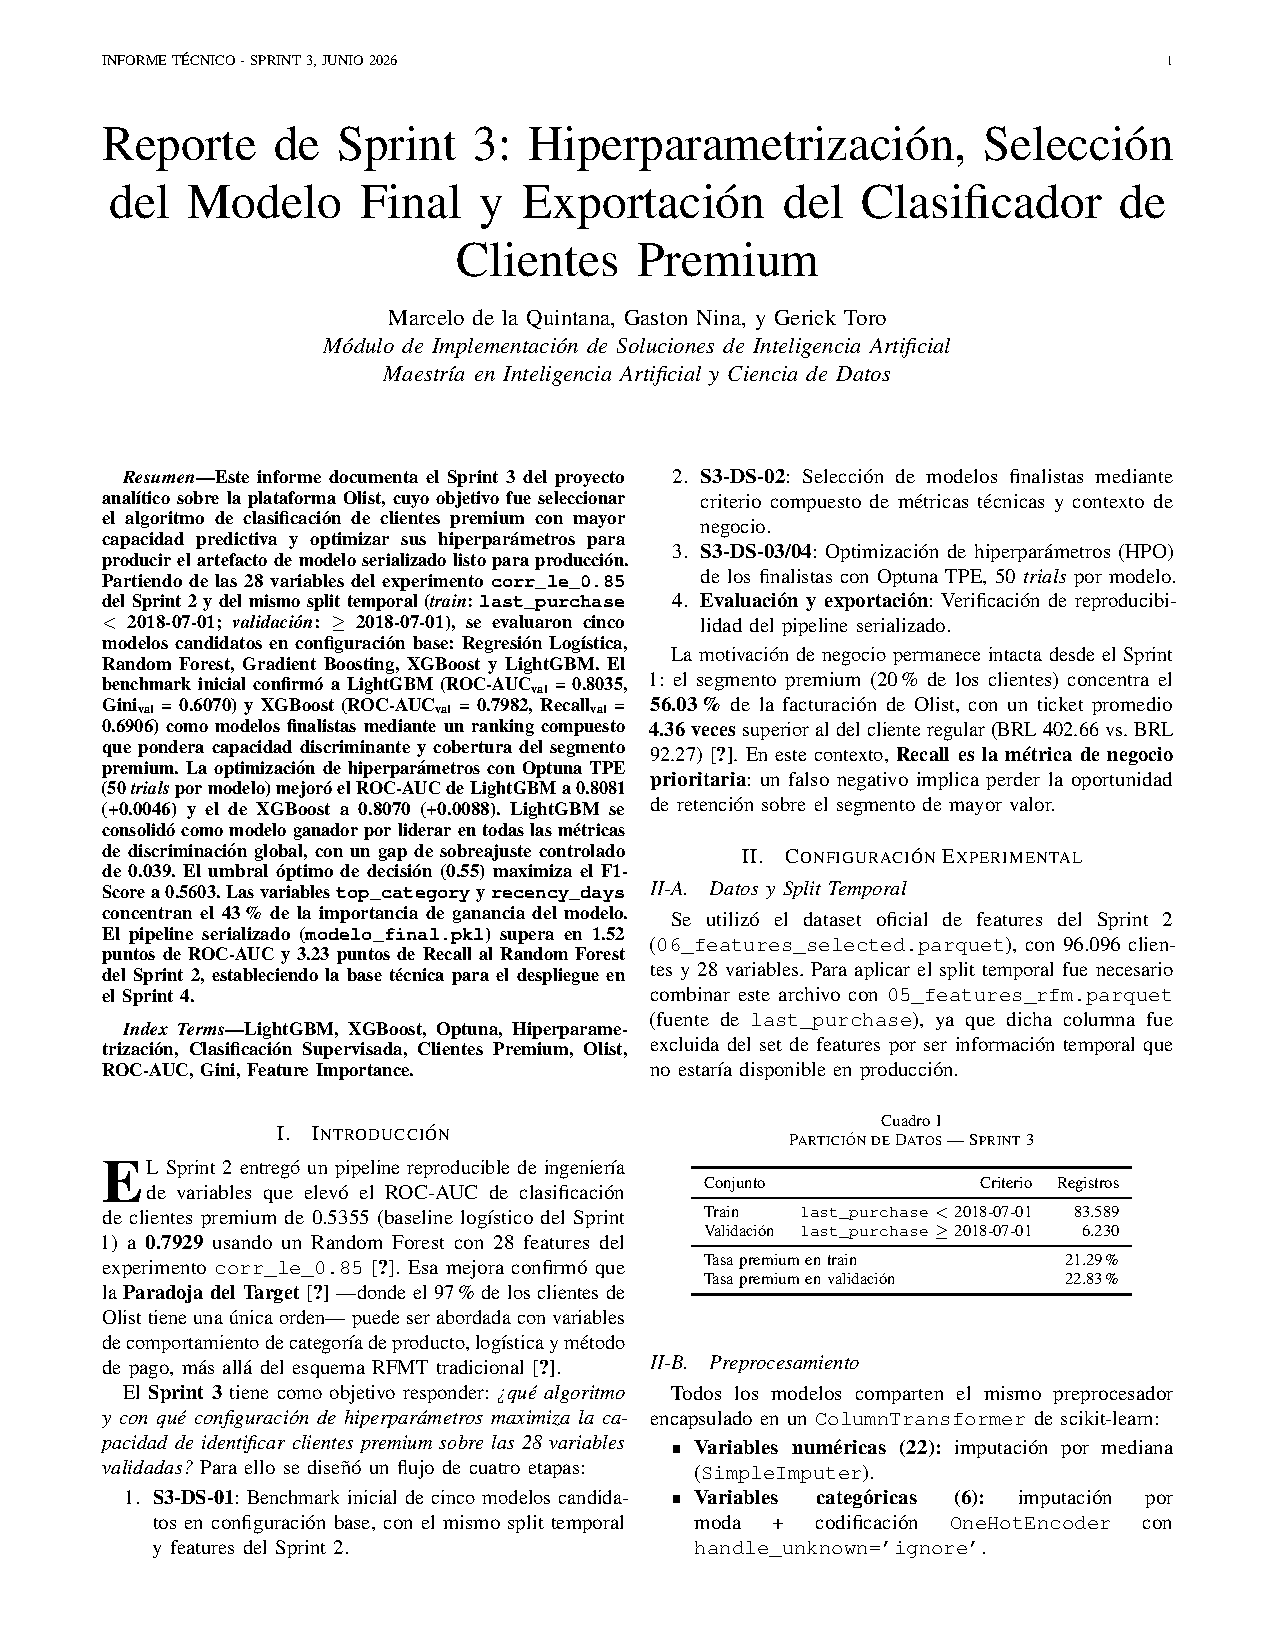
\includepdf[pages=-,pagecommand={}]{../../sprint_03/informes/sprint_03_reporte.pdf}

\section{Sprint 4: MVP, Backtest y Gobernanza}
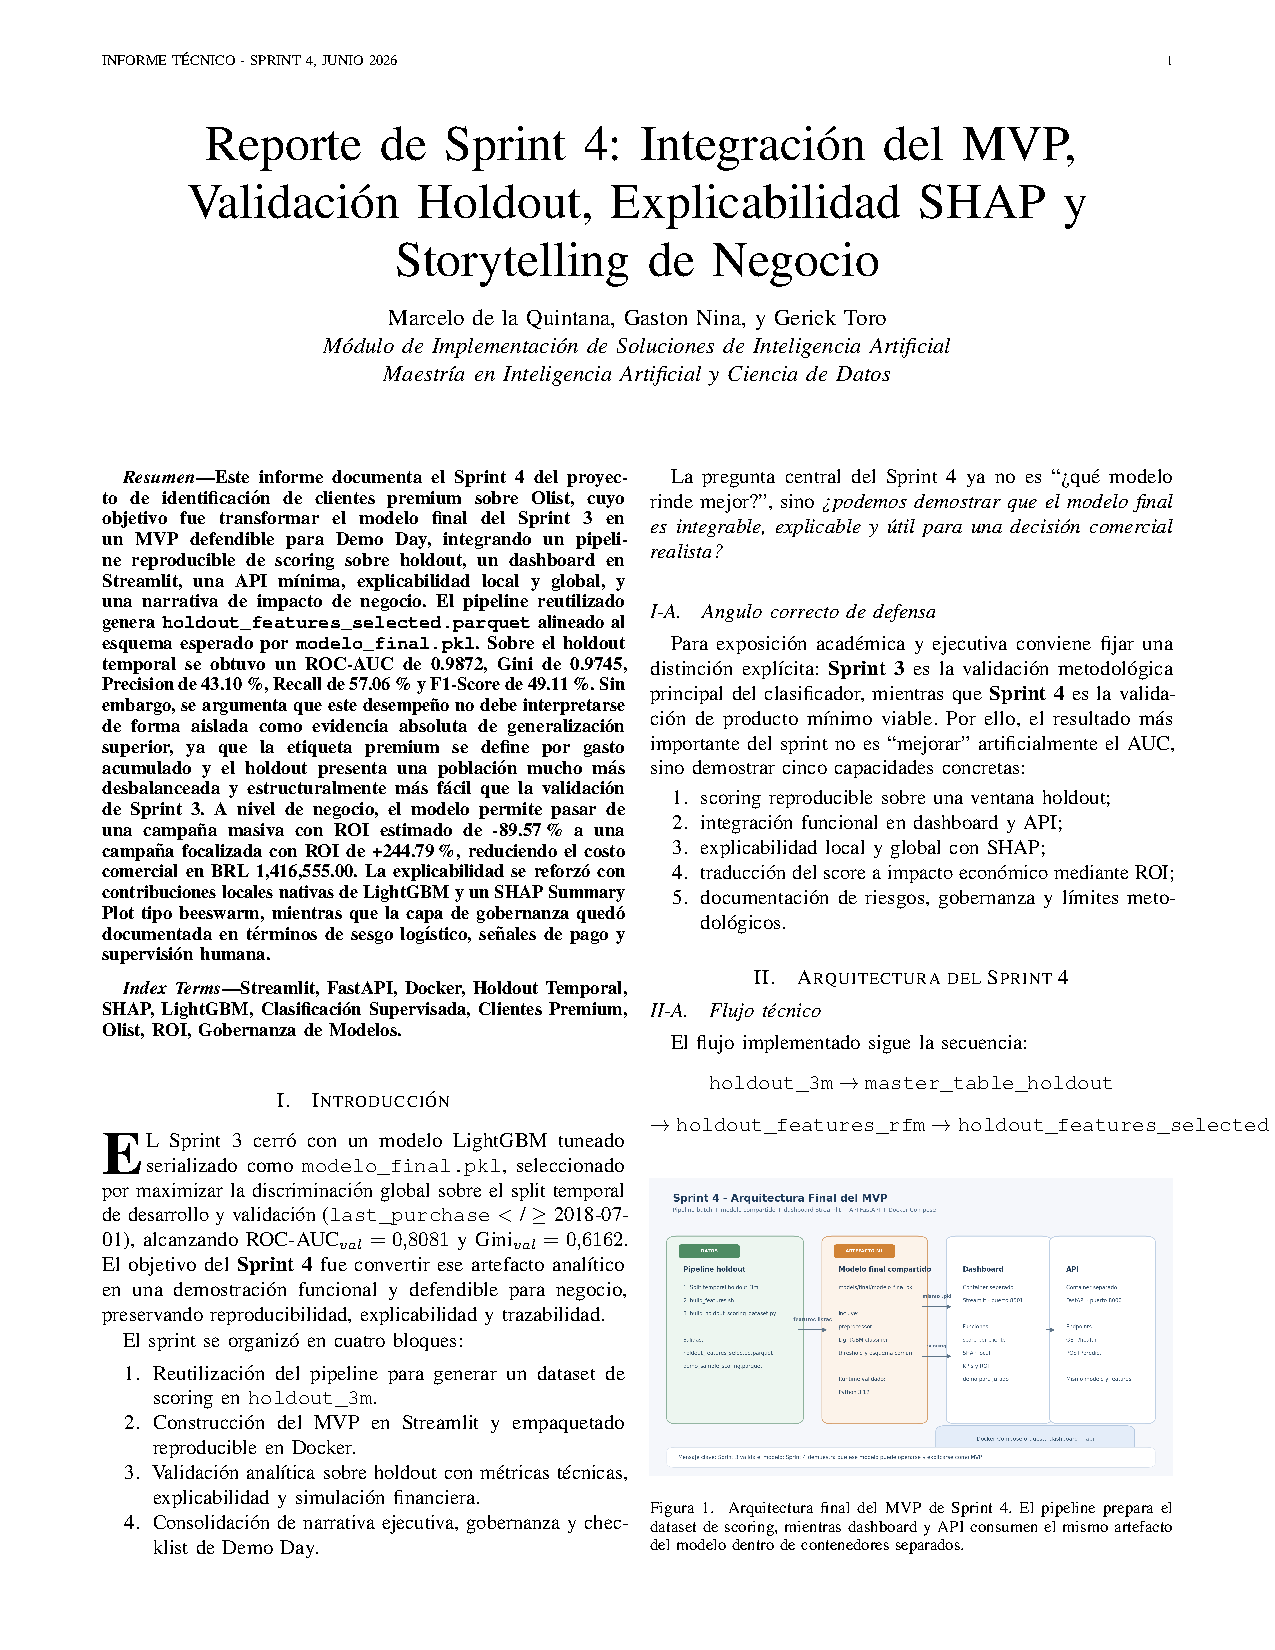
\includepdf[pages=-,pagecommand={}]{../../sprint_04/informes/sprint_04_reporte.pdf}

\end{document}
